% Статья про использование DSM-подхода для разработки средства программирования роботов QReal:Robots, часть большой статьи "Применение DSM-платформы QREAL при разработке среды программирования роботов QReal:Robots", скорее всего, для сборника кафедры.
% Идея: Есть подходящая для применения предметно-ориентированного подхода задача, есть DSM-платформа, применяем её для разработки визуального языка, пишем статью про то, как мы это делали, что получилось, и какие сделаны выводы.
% Фокус: Описание решения QReal:Robots как практического применения DSM-платформы QReal к реальной задаче. Что за задача, что мы получили от использования DSM-средства при её решении, что не смогли получить, но смогли реализовать вручную. Case study.
% Scope: Визуальное моделирование, DSM.
% Целевая аудитория: Специалисты, занимающиеся исследованиями в области DSM, технические специалисты, интересующиеся средствами программирования NXT.

\documentclass[a4paper]{article}
\usepackage[a4paper, top=17mm, bottom=17mm, left=17mm, right=17mm]{geometry}
\usepackage[utf8]{inputenc}
\usepackage[T2A,T1]{fontenc}
\usepackage[colorlinks,filecolor=blue,citecolor=green,unicode,pdftex]{hyperref}
\usepackage{cmap}
\usepackage[english,russian]{babel}
\usepackage{amsmath}
\usepackage{amssymb,amsfonts,textcomp}
\usepackage{color}
\usepackage[usenames,dvipsnames,svgnames,table]{xcolor}
\usepackage{array}
\usepackage{hhline}
\hypersetup{colorlinks=true, linkcolor=blue, citecolor=blue, filecolor=blue, urlcolor=blue, pdftitle=1, pdfauthor=, pdfsubject=, pdfkeywords=}
\usepackage{graphicx}
\usepackage{indentfirst}
\usepackage{cite}
\usepackage{literat}

\sloppy
\pagestyle{plain}

\title{Применение DSM-платформы QReal при разработке среды программирования роботов QReal:Robots}

\author{Ю.В.Литвинов \\ ст. преп. кафедры системного программирования СПбГУ, \\ инженер-программист ЗАО ``Ланит-Терком'' \\ yurii.litvinov@gmail.com}
\date{}

\begin{document}

\maketitle
\thispagestyle{empty}

\renewcommand{\thefootnote}{}
\footnote{\small{\copyright~Ю.В.Литвинов,~2012.}}
\renewcommand{\thefootnote}{\arabic{footnote}}
\setcounter{footnote}{0}

\begin{quote}
\small\noindent
В настоящее время в российских школах для преподавания информатики активно внедряются робототехнические конструкторы Lego Mindstorms NXT. Для программирования таких роботов обычно используются визуальные языки, но сред разработки, полностью удовлетворяющих  учителей и учеников, сейчас не существует. В данной работе представлен опыт разработки таких средств с помощью DSM-платформы QReal. В статье даётся краткий обзор архитектуры системы QReal, описывается созданный язык программирования роботов и роль DSM-средства QReal в процессе его создания. Делаются выводы о том, насколько эффективным оказался DSM-подход для решения поставленной задачи.
\end{quote}

\section*{Введение}
Сейчас в школах для преподавания информатики активно внедряются робототехнические конструкторы. Детям проще создавать свои первые программы, если они видят, как физический, осязаемый объект исполняет описанные в программе команды. Самым популярным на данный момент робототехническим набором является конструктор Lego Mindstorms NXT~\cite{legoNxt}(далее --- конструктор Lego). Он позволяет собирать из блоков управления, моторов и различных датчиков (датчики касания, расстояния, света и другие) несложные устройства, которые могут исполнять команды, посланные с компьютера по интерфейсу Bluetooth, или исполнять программу, загруженную на блок управления.

Для программирования конструктора Lego существует несколько сред программирования, например, NXT-G или Robolab~\cite{robolabHome}. Однако эти среды обладают рядом недостатков, затрудняющих их использование --- отсутствие полного перевода на русский язык, неудобный пользовательский интерфейс, недостаточная функциональность, высокая стоимость. Таким образом, существует потребность в разработке системы визуального программирования для конструкторов Lego, специально предназначенной для применения в российских школах.

На кафедре системного программирования Санкт-Петербургского Государственного Университета уже несколько десятилетий занимаются исследованиями в области визуальных языков и их применением в области разработки систем реального времени и встроенных систем~\cite{rtst1, rtst2, rtst3, videoDsl, dsmPlatforms, real1, real2, student1, student2, msfDsm, msfDsm2}. В частности, с 2007 года существует и активно развивается проект QReal~\cite{qReal}. В рамках этого проекта разрабатываются средства поддержки визуальных предметно-ориентированных языков (Domain-Specific Modelling, DSM-подход). Поскольку разработка визуального языка программирования роботов и соответствующих программных средств поддержки является интересной областью для использования предметно-ориентированного подхода, было решено применить результаты проекта QReal для решения этой задачи.  

С научной точки зрения программирование роботов является интересной предметной областью для апробации DSM-подхода. С одной стороны, использование визуальных языков программирования довольно широко распространено среди людей, занимающихся робототехникой, поэтому здесь можно рассчитывать на содержательное сравнение с существующими решениями и обратную связь от пользователей, уже знакомых с различными визуальными решениями. С другой стороны, программирование роботов --- достаточно узкая предметная область, поэтому можно получить заметное преимущество от специализированного языка. Вместе с тем эта область достаточно содержательна, поэтому такой язык является нетривиальным. Типичные программы для роботов состоят из элементарных команд, таких как ``включить моторы'', ``ожидать такое-то показание сенсора'' и т.д., и управляющих конструкций, таких как условные операторы и циклы. На языке общего назначения такие команды были бы вызовами программного интерфейса (Application Programming Interface, далее --- API) операционной системы или библиотек робота и требовали бы для себя различных вспомогательных конструкций, таких как операторы включения и объявления переменных, а на специализированном языке каждая такая команда представляется одним блоком, для использования которого достаточно просто разместить его на диаграмме. Это существенно снижает требования к знаниям программиста и снижает вероятность ошибки в программе --- например, невозможно ошибиться при указании имени вызываемой функции. Вместе с тем многие языковые конструкции, типичные для императивного программирования, такие как ветвления и циклы, будут присутствовать и в этом языке, так что если удастся подобрать удобное графическое представление для программ для роботов, можно надеяться обобщить полученный результат на другие задачи, хорошо выражаемые в императивных терминах.

В статье описано, с какими трудностями пришлось столкнуться в ходе разработки визуальной среды программирования конструктора Lego, чем помог DSM-инструментарий, а в чём он не смог помочь. Изложенные в статье результаты могут быть интересны тем, что разрабатываемую с помощью DSM-инструментария систему удалось довести до состояния, в котором её смогли успешно использовать люди, занимающиеся робототехникой и далёкие от программирования, в том числе и ученики пятых-шестых классов. 

\section{Средства визуального программирования роботов}
Cуществует довольно много сред программирования роботов Lego, в том числе и визуальных. Наиболее популярными на данный момент являются среды NXT-G, Robolab~\cite{robolab}, Microsoft Robotics Developer Studio~\cite{mrds}.

Среда NXT-G поставляется в комплекте с конструктором Lego Mindstorms NXT, базируется на системе LabView (системе, предназначенной для моделирования и обработки данных научных экспериментов), и имеет модель вычислений, ориентированную на данные. Язык NXT-G  состоит из блоков, блоки имеют входы и выходы, блок начинает выполнение, когда на всех его входах есть готовые данные. Такой подход отличается от принятого в классических блок-схемах, однако распространён в средствах, используемых учёными и инженерами, а также в автоматном программировании ~\cite{shalito1, shalito2}.  NXT-G имеет ряд существенных недостатков, например, слабую поддержку математических выражений: каждая элементарная операция представляется отдельным блоком, что требует от пользователя, фактически, рисовать дерево разбора арифметического выражения. Таким образом, даже такая несложная и широко используемая конструкция, как пропорциональный регулятор, на NXT-G будет выглядеть очень объёмно и сложно.

Среда Robolab~\cite{robolab} так же, как и NXT-G, базируется на LabView и использует ту же модель вычислений, однако, позволяет писать математические выражения текстом. Поэтому среда Robolab гораздо шире распространена среди людей, серьёзно увлекающихся робототехникой. Интересная особенность этой среды заключается в том, что она специально создавалась для образовательных целей. Robolab  поддерживает несколько уровней использования. На самом первом уровне пользователю предоставляется готовый шаблон программы, где он может только выбрать, с какого сенсора считать данные и на какой мотор послать команду. А на последнем уровне пользователь может произвольным образом комбинировать более 400 блоков языка, используя ветвления, циклы, параллельное исполнение, подпрограммы и т.д. Таким образом, система полезна как дошкольникам, так и старшеклассникам. Пользовательский интерфейс Robolab выглядит устаревшим, а сама среда довольно дорога, поэтому у многих школьных учителей есть желание отказаться от Robolab в пользу чего-нибудь более современного, но пока у Robolab не существует серьёзных конкурентов.

Среда Microsoft Robotics Developer Studio (MRDS)~\cite{mrds} гораздо мощнее и сложнее рассмотренных выше продуктов. Она создавалась как средство визуального программирования сложных многопоточных приложений с реактивным поведением, которые могут применяться не только в робототехнике, но и во многих других областях, например, для программирования серверного ПО для крупных Web-сайтов. Язык визуального программирования VPL (Visual Programming Language), используемый в MRDS, по сути, визуализирует связи по данным между отдельными параллельно исполняемыми компонентами (Web-сервисами), из которых состоит программа. Такой подход требует больших вычислительных ресурсов (больше, чем среды, описанные выше), поэтому MRDS может управлять роботом Lego только дистанционно, исполняя программу на компьютере. Сама среда ориентирована на более дорогие роботы, имеющие в своё составе полноценный компьютер (например, в документации к MRDS описана ``стандартная модель’’ робота --- трёхколёсная платформа с установленным на ней ноутбуком, сенсором Microsoft Kinect\textregistered, инфракрасными датчиками расстояния и сонаром). Среда ориентирована на студентов и профессиональных программистов, начинающим знакомиться с робототехникой использовать её сложно. Кроме того, используемая модель вычислений слишком специфична, чтобы быть полезной в качестве иллюстративного материала при преподавании робототехники и программирования.

Таким образом, можно сделать вывод о том, что существующие среды, кроме Robolab, слабо подходят для преподавания в российских школах. Среда Robolab также имеет ряд существенных недостатков. Таким образом, существует потребность в создании свободно распространяемой среды программирования, схожей по функциональности с Robolab, но обладающей рядом дополнительных возможностей, таких как средства отладки, генерация кода, полноценная русификация.

\section{Предметно-ориентированное моделирование}
Предметно-ориентированное визуальное моделирование --- перспективный и развивающийся сегодня подход к разработке программного обеспечения. Его суть заключается в том, что прикладная задача решается не с помощью языка общего назначения, такого как C++, Java, C\#, UML, а с помощью узкоспециализированного визуального языка, специально созданного для решения задач в данной предметной области или даже для решения одной  задачи. Узкая направленность языка позволяет эффективно создавать на нём законченные программы, не требующие модификаций на текстовых языках программирования. Специализированный язык близок к предметной области, и это позволяет использовать его даже людям, не владеющим программированием. 

Для создания предметно-ориентированного решения  требуется небольшой коллектив высококвалифицированных программистов и аналитиков. По окончании разработки этим решением может пользоваться большое количество обычных программистов, либо экспертов предметной области, что обходится дешевле, чем разработка системы традиционными средствами. Кроме визуальных существуют хорошо известные текстовые предметно-ориентированные языки, такие как SQL, AWK, а также языки описания грамматик в конструкторах компиляторов. Исследования~\cite{kelly, kieburtz, weiss} сообщают о росте производительности труда программиста в 3--10 раз при использовании предметно-ориентированных языков по сравнению с программированием на текстовых языках общего назначения.

Разумеется, создавать специальный визуальный язык и разрабатывать для него индустриальные средства ``вручную’’ было бы весьма не просто. Создание хорошей CASE-системы ``с нуля’’ под силу только компаниям, которые на этом специализируются, и оправдано только в том случае, если эта CASE-система будет продаваться как коробочный продукт для массового покупателя, что противоречит самой идее предметно-ориентированного моделирования. Поэтому активно развиваются специальные инструменты для быстрого создания визуальных языков и средств их инструментальной поддержки, так называемые DSM-платформы~\cite{dsmPlatforms}. Любая такая платформа позволяет в том или ином виде описать синтаксис визуального языка и автоматически (или полуавтоматически) создать для него визуальный редактор. Некоторые DSM-платформы также позволяют задать для визуального языка правила генерации в текстовый целевой язык, описать набор доступных для языка инструментов и т.д. Наиболее зрелыми на данный момент DSM-платформами являются Eclipse Graphical Modelling Project~\cite{gmp, sorKoz}, MetaEdit+~\cite{metaEditPlus}, Visual Studio Visualization and Modeling SDK~\cite{vsvmsdk}, Microsoft Visio~\cite{visio}. 

Платформа Graphical Modelling Project (GMP) --- набор проектов в области визуального моделирования. Самыми зрелыми являются продукты Eclipse Modeling Framework (библиотека для работы с метамоделями/моделями с помощью API, а также в текстовом виде) и Graphical Editing Framework (библиотеки для редакторов графов)~\footnote{Обзор GMP на русском языке можно  найти в работе~\cite{sorKoz}}. GMP является мощной платформой и  позволяет создавать отчуждаемые визуальные редакторы и генераторы кода, позволяя задавать метамодель языка в том числе с помощью стандарта обмена метамоделями XMI~\cite{xmi}, имеет открытый исходный код и распространяется свободно, являясь де-факто стандартом для осуществления научных исследований. С её помощью можно легко получить простой графический редактор для несложного визуального языка, но когда возникают более-менее нестандартные требования, то использование технологии оказывается очень сложным~\footnote{Об опыте использования графических технологий Eclipse в российских разработках см., например, работу ~\cite{shalitoEcl}.}. 

DSM-платформа MetaEdit+ является наиболее зрелой на данный момент и активно используется в промышленном программировании. Она имеет свой метаязык и графический редактор для описания абстрактного синтаксиса визуального языка, а также редактор формы элементов для задания конкретного синтаксиса и текстовый язык описания правил генерации целевого кода. MetaEdit+ позволяет создавать отдельно работающие редакторы. Её основными недостатками являются высокая цена и то, что исходные коды этой системы закрыты.

Visual Studio Visualization and Modeling SDK (бывший Microsoft DSL Tools) позволяет создавать визуальные редакторы, встраиваемые в среду Microsoft Visual Studio 2010. На нём довольно удобно описывать простые визуальные языки, однако, если требуется что-либо нестандартное (например, нестандарные фигуры элементов), то требуется ручное кодирование на языке C\#. Распространяется продукт бесплатно, но может применяться только в составе среды Visual Studio, стоимость которой довольно велика. Кроме того, получающиеся в итоге графические редакторы также неразрывно связаны с Visual Studio.

Среда Microsoft Visio позиционируется разработчиками скорее как векторный графический редактор, чем как DSM-платформа, однако содержит средства описания новых фигур и полноценный API и средства интеграции с Visual Studio, что даёт возможность использовать её в качестве легковесной DSM-платформы. Использование её в таком качестве оказалось удобным в том числе и в коммерческих проектах~\cite{videoDsl}. Однако же, Visio не обладает всей необходимой для DSM-платформы функциональностью --- нет полноценных средств описания метамодели, недостаточно функциональный программный интерфейс, затрудняющий работу с диаграммами сторонних инструментов, сложности с созданием нетривиальных фигур, нет разделения на модель и представления (vsd-файлы хранят диаграммную и модельную информацию вместе, что сильно затрудняет программную обработку моделей в Visio). 


\section {Cистема QReal}
Кроме упомянутых выше известных и зрелых DSM-платформ существует и некоторое количество академических разработок. Одна из таких разработок --- платформа QReal~\cite{qReal}, созданная на кафедре системного программирования Санкт-петербургского государственного университета. QReal --- это метаCASE-система, разрабатываемая как проект с открытым исходным кодом~\cite{qRealGithub}. На данный момент система QReal обладает следующими возможностями.
\begin{itemize}
  \item Средства для задания метамодели визуального  языка в специальном XML-формате, либо в графической форме. Соответствующий редактор сам реализован как предметно-ориентированный язык, существует его метамодель в виде XML-описания и для него применимы все возможности QReal, применимые к другим визуальным языкам.
  \item Средства для задания формы фигур визуального языка с помощью встроенного графического редактора форм, представляющего собой простой векторный графический редактор с поддержкой возможности отображать значения логических свойств элемента прямо на фигуре. В качестве альтернативы есть возможность задавать форму фигуры непосредственно в XML-файле метамодели, в формате, похожем на стандарт векторной графики SVG.
  \item Средства автоматической генерации кода редактора по метамодели и описаниям форм фигур. Редактор генерируется как подключаемый модуль на языке C++ и подгружается в среду QReal сразу по окончании генерации и сборки. Имея собранный редактор, метаредактор можно отключить и использовать QReal как независимый редактор предметно-ориентированного языка.
  \item Репозиторий, в котором хранятся все данные создаваемых пользователем моделей. Этими данными могут пользоваться как подключаемые модули QReal, так и сторонние приложения, которые могут подключать репозиторий как динамически загружаемую библиотеку.
  \item Программный интерфейс для подключаемых модулей-инструментов, открывающий доступ как к репозиторию, так и к общей функциональности системы, такой как вывод ошибок пользователю и подсветка элементов на диаграмме. Интерфейс позволяет создавать инструменты ``вручную’’, на C++, и реализовывать с их помощью генераторы кода, средства возвратного проектирования, интерпретаторы моделей, различные валидаторы и т.д.
\end{itemize}

\section{Визуальный язык QReal:Robots}
Визуальный язык программирования роботов, используемый в QReal:Robots, основывается на абстракции потока управления. Язык состоит из блоков, представляющих элементарные команды роботу, такие как ``включить моторы на указанных портах с указанной мощностью на указанное количество оборотов’’, и связей, показывающих передачу управления от одного блока к другому. В момент выполнения программы существует один или несколько маркеров выполнения. Блок, получивший маркер, выполняет свои команды и отдаёт маркер блоку, с которым связан соединительной линией. Пример программы приведён на рисунке~\ref{programExample}.

\begin{figure} [ht]
  \begin{center}
    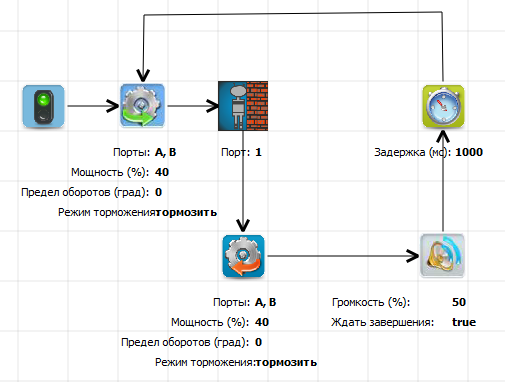
\includegraphics[width=0.7\textwidth]{programExample.png}
    \caption{Пример программы QReal:Robots}
    \label{programExample}
  \end{center}
\end{figure}

Все блоки языка делятся на несколько крупных смысловых групп, которые могут быть отдельно свёрнуты/развёрнуты в палитре. В языке присутствуют следующие блоки.
\begin{itemize}
	\item Алгоритмы --- блоки для организации диаграмм и управления вычислительным процессом.
  \begin{itemize}
    \item Диаграмма поведения робота --- позволяет создавать новые диаграммы. В каждый конкретный момент времени может быть выполнена или сгенерирована только одна диаграмма, но проект может содержать несколько диаграмм, между которыми можно переключаться.
    \item Линия соединения --- задаёт последовательность передачи управления между блоками.
    \item Параллельные задачи --- позволяет разделить поток управления на несколько параллельных потоков, которые будут исполняться независимо. Выглядит как блок, из которого выходит несколько соединительных линий, который при получении маркера управления создаёт несколько маркеров (по одному для каждой соединительной линии) и отправляет их каждому соединённому с ним блоку. После разделения задачи независимы.
    \item Условие --- оператор, проверяющий заданное логическое условие и, в зависимости от исхода проверки, передающий маркер управления на одну из двух исходящих соединительных линий. Поскольку в QReal, в отличие от LabView, у блока нет понятия ``порт’’ в том смысле, что все исходящие линии равнозначны, одна из них должна быть помечена условием, по которому выполняется переход, а вторая должна быть не помечена. По непомеченной связи управление передаётся в том случае, если условие не выполнено.
    \item Цикл --- блок для задания аналога цикла ``for’’ в текстовых языках. Блок должен иметь две исходящие связи, по одной из которых передаётся управление до тех пор, пока выполняется цикл. Когда цикл заканчивается, то управление передаётся по второй связи. Количество итераций задаётся как параметр блока.
  \end{itemize}
  \item Действия --- команды роботу.
  \begin{itemize}
    \item Гудок --- команда роботу издать звук.
    \item Играть звук --- команда роботу издать звук заданной частоты и громкости. Отличается от блока ``Гудок’’ существенно большими возможностями в настройке.
    \item Моторы вперёд --- команда роботу включить моторы на заданных портах с заданной мощностью на заданное количество оборотов. Если число оборотов указано как 0, моторы будут работать неограниченно.
    \item Моторы назад --- команда роботу включить моторы в режиме движения назад с параметрами, аналогичными параметрам блока ``Моторы вперёд’’.
    \item Моторы стоп --- команда роботу выключить моторы.
    \item Функция --- блок для записи произвольного математического выражения или кода на С.
  \end{itemize}
  \item Инициализация --- блоки, отвечающие за инициализацию робота и начало работы программы.
  \begin{itemize}
    \item Блок инициализации --- блок, обозначающий начало программы и позволяющий задать, на каком порту находится какой сенсор.
    \item Конец --- блок, обозначающий конец программы и отключение моторов и сенсоров робота.
    \item Начало --- блок, аналогично блоку инициализации и обозначающий начало программы, но без параметров.
    \item Сбросить показания энкодеров --- блок, обнуляющий значения счётчиков оборотов моторов.
  \end{itemize}
  \item Ожидания --- блок, передающий управление дальше только при наступлении какого-либо события.
  \begin{itemize}
    \item Ждать интенсивность цвета --- блок, продолжающий выполнение программы только в том случае, если значение, возвращаемое сенсором цвета на заданном порту, будет больше или меньше заданного значения.
    \item Ждать свет --- блок, продолжающий выполнение программы, если значение, возвращаемое сенсором освещённости на заданном порту, будет больше или меньше заданного значения.
    \item Ждать сенсор касания --- выполнение программы продолжается при срабатывании сенсора касания на заданном порту.
    \item Ждать сонар --- выполнение программы продолжается, если значение, которое вернул ультразвуковой сенсор расстояния, больше или меньше указанного значения.
    \item Ждать цвет --- выполнение программы будет продолжено, если сенсор цвета обнаружит заданный цвет.
    \item Ждать энкодер --- выполнение продолжится, если значение счётчика оборотов на указанном порту будет больше заданного.
    \item Таймер --- выполнение продолжится по истечении указанного промежутка времени (в миллисекундах).
  \end{itemize}
\end{itemize}

Язык позволяет везде, где можно задавать численные параметры, использовать математические выражения, включающие в себя арифметические действия, тригонометрические функции и переменные. Кроме того, имеется специальный блок ``Функция’’, используемый для работы с математическими выражениями. В выражениях можно использовать текущие показания с помощью так называемых сенсорных переменных --- предопределённых переменных с именами Сенсор1, Сенсор2 и т.д., значения которых обновляются в соответствии с показаниями сенсоров. Пример программы, использующей математические выражения и сенсорные переменные, приведён на рисунке~\ref{movingAlongTheLine}. На этом рисунке приведена реализация алгоритма движения робота вдоль чёрной линии на полу по показаниям двух датчиков освещённости на основе пропорционально-дифференциального регулятора (подробнее см., например, в~\cite{filippov}).

\begin{figure} [ht]
  \begin{center}
    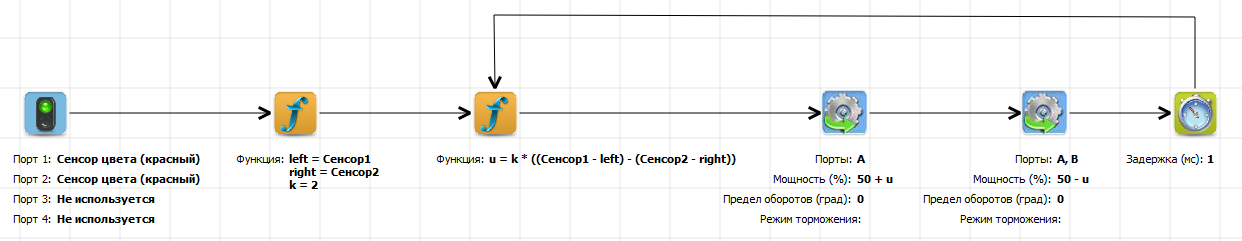
\includegraphics[width=\textwidth]{movingAlongTheLine.png}
    \caption{Алгоритм движения робота вдоль линии}
    \label{movingAlongTheLine}
  \end{center}
\end{figure}

Язык QReal:Robots можно рассматривать как типичный пример визуального предметно-ориентированного языка. Важно, что программа на визуальном языке понятна даже такому пользователю, который впервые видит этот язык, но имеет некоторый опыт в программировании роботов. Для этого используется такой приём, как отображение блоков языка в виде картинок, понятных людям, которые ориентируются в предметной области (описанный, например, в~\cite{theBook}). Так блоки, управляющие моторами, изображаются в виде  моторов из конструктора Lego NXT, и все, кто хоть немного знаком с этим конструктором, по внешнему виду блока смогут понять его предназначение. Кроме того, оказалось важным, что передача управления между блоками изображается стрелками --- это делает программу ещё более наглядной.

\section{Инструментальные средства QReal:Robots}
С помощью QReal оказалось легко создать визуальный язык, но инструментальные средства для него необходимо создавать ``вручную’’ --- управление реальным роботом по Bluetooth, двухмерная модель робота и т.д. 

Инструментальная поддержка программирования роботов в QReal:Robots состоит из двух частей: интерпретатора диаграмм и генератора кода на языке C для загрузки программы на робот. Интерпретатор создавался с учётом следующих требований.
\begin{itemize}
  \item Возможность быстро задавать поведение для новых блоков визуального языка.
  \item Интерпретация диаграмм передачей роботу команд по Bluetooth или USB, в зависимости от выбора пользователя.
  \item Наличие двухмерной модели робота, которая могла бы интерпретировать диаграмму вместо реального робота. Двухмерная модель робота должна взаимодействовать с симулируемым окружением --- должно быть возможно нарисовать стены, линии и цветные области на полу.
  \item Архитектура должна позволять быстро поддержать новые виды оборудования, например, нестандартные сенсоры.
\end{itemize}

Архитектура интерпретатора приведена на рисунке~\ref{interpreterArchitecture}.

\begin{figure} [ht]
  \begin{center}
    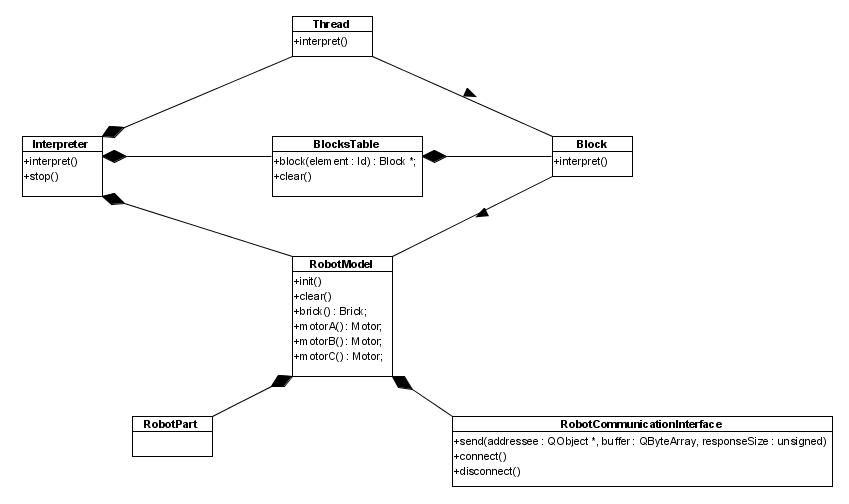
\includegraphics[width=0.7\textwidth]{interpreterArchitecture.jpg}
    \caption{Архитектура интерпретатора}
    \label{interpreterArchitecture}
  \end{center}
\end{figure}

Процесс интерпретации диаграммы начинает класс Interpreter, который хранит в себе контекст вычислений и контролирует потоки запущенной программы. Первое, что он делает --- обходит переданную на интерпретацию диаграмму, создавая для каждого блока объект, обеспечивающий его выполнение. При этом заполняется таблица блоков BlocksTable, ставящая в соответствие каждому идентификатору элемента на диаграмме такой объект, чтобы в дальнейшем иметь возможность быстро найти объект-исполнитель для передачи управления. После этого создаётся основной поток программы, содержащий в себе маркер исполнения. Маркер устанавливается на блок начала или инициализации, после чего проводится инициализация логической модели робота (класс RobotModel, в зависимости от настроек, может реализовывать как управление реальным роботом, так и управление двухмерной моделью, для этого используется шаблон ``стратегия’’). После того, как инициализация закончена (для этого может потребоваться дождаться ответа от робота об инициализации оборудования), запускается метод interpret() блока, который хранит маркер выполнения. Блок выполняется (для этого снова может потребоваться асинхронная посылка команд на робот и ожидание ответа) и после этого сообщает своему потоку, на какой следующий блок следует передать маркер управления. Так продолжается до тех пор, пока маркер управления потока не доходит до блока ``Конец’’, и после этого поток завершается.

Взаимодействие с реальным роботом осуществляется через реализацию интерфейса RobotCommunicationInterface, который предоставляет возможность послать роботу заданный пакет байтов. Роботы Mindstorms NXT позволяют управлять собой с помощью команд по Bluetooth и по USB, поэтому в QReal:Robots имеется две реализации RobotCommunicationInterface. Управление по Bluetooth осуществляется через виртуальный COM-порт Bluetooth-соединения, обеспечиваемый средствами операционной системы, а управление по USB требует наличия установленного драйвера робота, и команды посылаются роботу через этот драйвер. Каждый блок диаграммы реализован в терминах логической модели робота, логическая модель в случае взаимодействия с реальным роботом формирует управляющую команду и посылает её роботу через RobotCommunicationInterface. В случае с двухмерной моделью логическая модель вызывает методы классов, реализующих двухмерную модель, которые отрабатывают команды и формируют значения сенсоров.

Двухмерная модель моделирует робот с жёстко заданным расположением моторов, однако позволяет настраивать расположение сенсоров. Поддерживаются сенсоры касания, расстояния, цвета. Двухмерная модель позволяет рисовать стены, линии и цветные области на полу. Внешний вид окна двухмерной модели представлен на рисунке~\ref{2dModel}.

\begin{figure} [ht]
  \begin{center}
    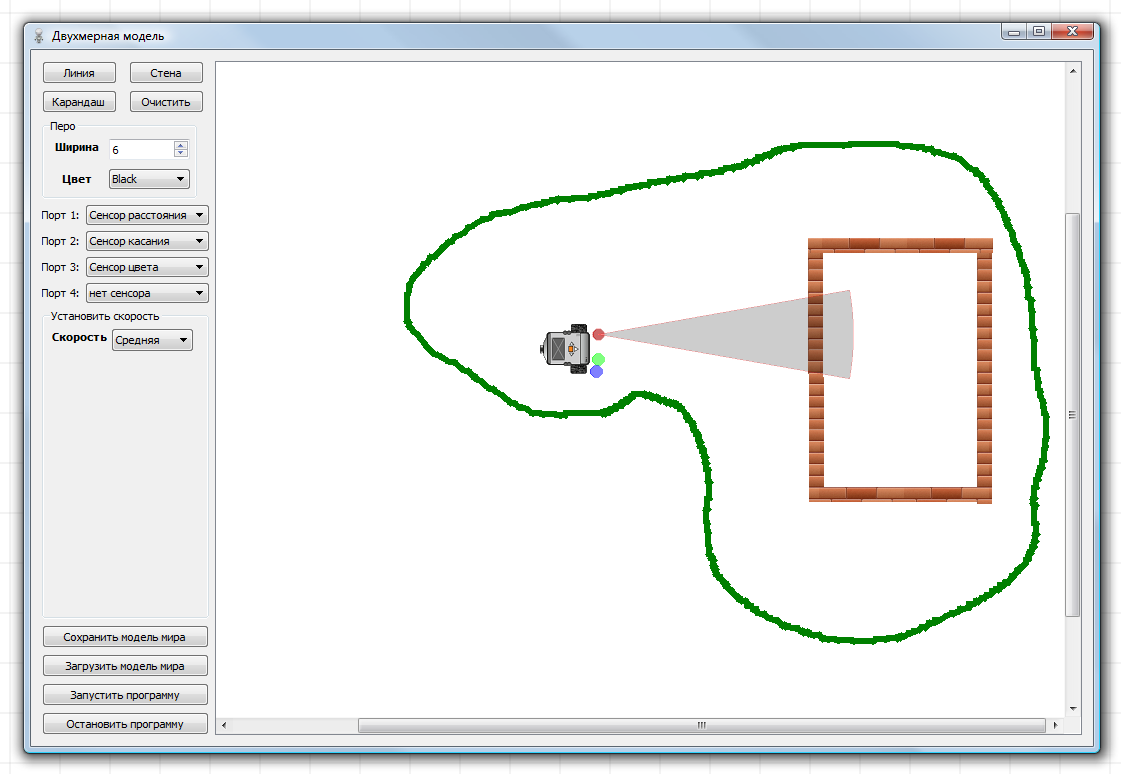
\includegraphics[width=0.7\textwidth]{2dModel.png}
    \caption{Окно двухмерной модели}
    \label{2dModel}
  \end{center}
\end{figure}

Генератор кода на C в QReal:Robots реализован в виде отдельной компоненты, которая может подключаться к основной программе независимо от интерпретатора. В качестве среды времени исполнения (runtime) генератор использует операционную систему nxtOSEK~\cite{nxtOsek}, одну из самых быстрых доступных на данный момент операционных систем для роботов Lego. Генератор порождает c-файл с кодом решения задачи и oil-файл с настройками параметров выполнения кода. Далее автоматически запускается кросскомпилятор из состава nxtOSEK, собирающий эти файлы вместе с заголовочными файлами операционной системы, после чего получившийся бинарный образ передаётся роботу по USB посредством утилиты, распространяемой с драйвером робота. Для пользователя этот процесс прозрачен, достаточно подключить робот, нажать кнопку ``Загрузить программу на робот’’, и после этого сгенерированный по диаграмме код программы покажется в окне встроенного в QReal текстового редактора, и одновременно начнётся процесс компиляции и загрузки программы.

Технически генератор реализован по шаблонной схеме, довольно типичной для генераторов кода по диаграммам в DSM-подходе~\cite{theBook}. Имеется шаблон порождаемого исходного кода, представляющий из себя почти готовую программу со специально размеченными местами, куда надо вставить код, сгенерированный по диаграмме. При генерации кода могут использоваться вспомогательные шаблоны --- как правило, небольшие фрагменты программы, параметризуемые информацией из диаграммы. Небольшой пример шаблона приведён ниже:
\begin{verbatim}
void ecrobot_device_initialize(void)
{
@@INITHOOKS@@
}
\end{verbatim}
Здесь на место \verb|@@INITHOOKS@@| вставляется код, сгенерированный по блоку инициализации диаграммы, а всё остальное попадает в выходной файл без изменений. По каждому блоку генерируется свой небольшой фрагмент программы, при этом некоторую сложность представляют структурные операторы, например, циклы или условные переходы. Проблема в том, что диаграмма может быть нарисована неструктурно, синтаксис визуального языка не запрещает этого: например, условный переход внутрь цикла, или условный переход наружу из оператора if. С точки зрения визуального языка такие ситуации абсолютно корректны, но в текcтовое представление переводятся только с использованием операторов goto (или техник goto elimination, известных в реинжиниринге). Однако, поскольку сгенерированный код предполагается использовать в иллюстративных целях, использовать оператор goto было бы крайне нежелательно. Генератор применяет набор эвристик, позволяющих найти на диаграмме фрагменты, соответствующие структурным операторам if, циклам while и do/while. В случае, если генератор не может породить структурный код по данной диаграмме, выдаётся ошибка и код не порождается вообще. Интерпретация такой диаграммы, тем не менее, вполне возможна.

\section{Опыт применения QReal}
\subsection{Создание графического редактора}
Визуальный язык для QReal:Robots создавался с помощью метаредактора QReal. Полная метамодель одной из версий языка представлена на рисунке~\ref{robotsMetamodel}. Как видно, она целиком помещается на одном экране. Все элементы также имеют свойства (в том числе, внешний вид), которые на рисунке не показаны.

\begin{figure} [ht]
  \begin{center}
    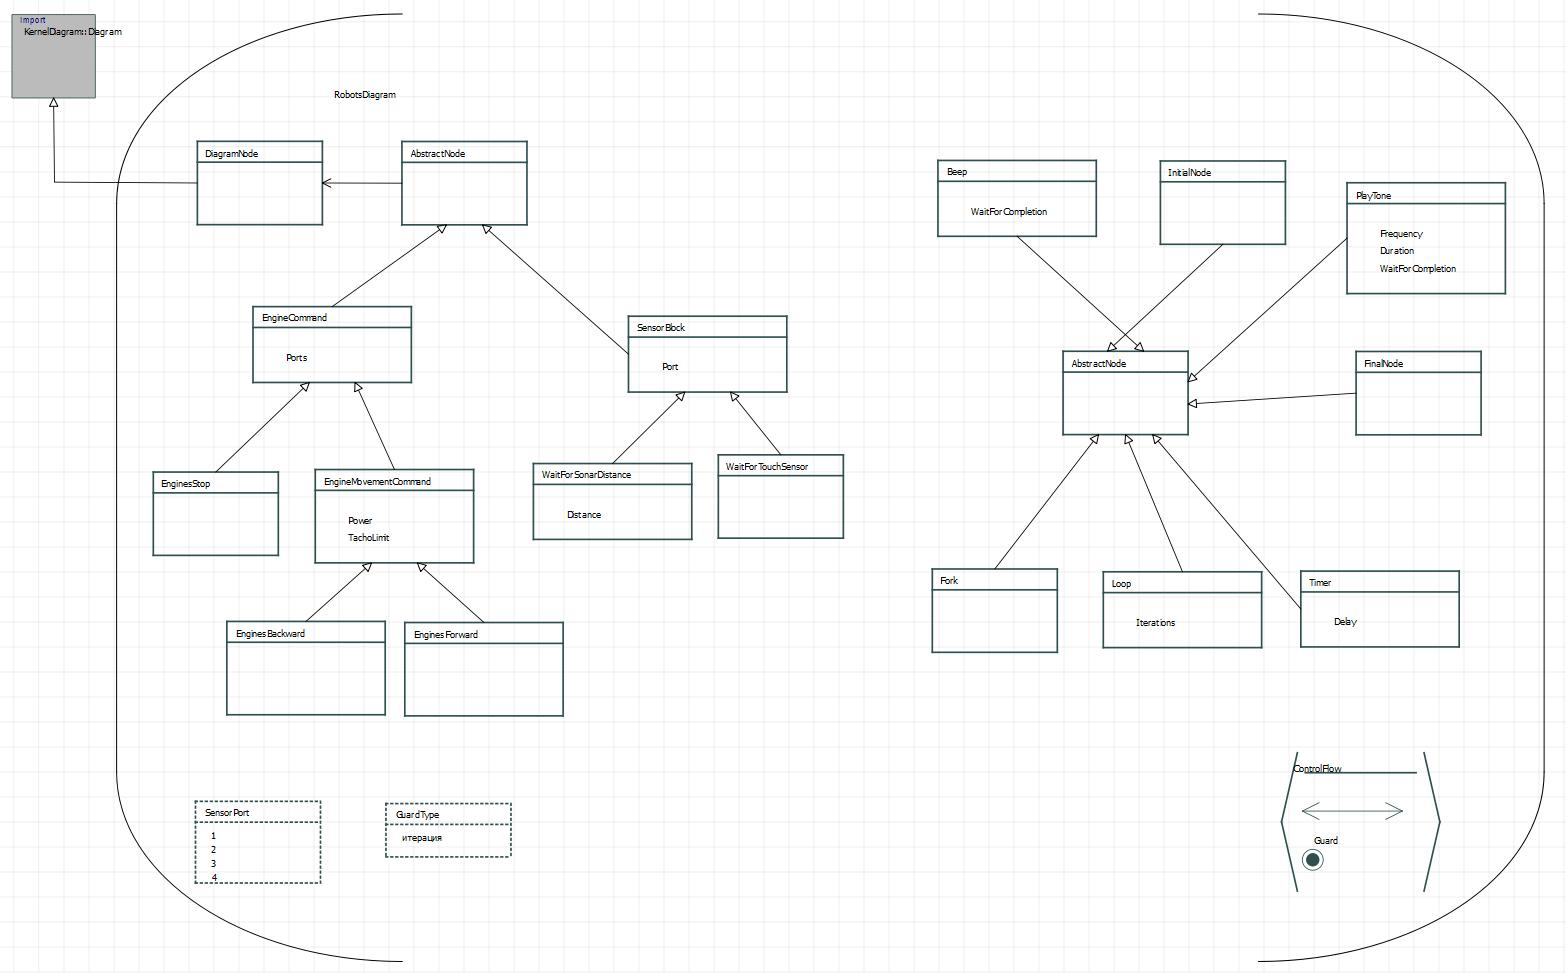
\includegraphics[width=\textwidth]{robotsMetamodel.jpg}
    \caption{Метамодель языка QReal:Robots}
    \label{robotsMetamodel}
  \end{center}
\end{figure}

Корневой сущностью метамодели является диаграмма, на неё помещаются все элементы языка. Диаграмма --- это вкладка в палитре блоков, на неё добавляются все блоки языка, все виды связей, все перечислимые типы, используемые в свойствах элементов, и т.д. Одна метамодель может содержать несколько диаграмм, тогда плагин-редактор, сгенерированный из этой метамодели, при загрузке будет добавлять несколько вкладок в палитру. Внутри диаграммы находятся узлы --- элементы визуального языка. Узлы могут быть связаны отношением наследования и отношением ``содержи’’. Последнее указывает, что один узел может содержать другой в себе, то есть являться контейнером для этого узла. В языке программирования роботов узел ``диаграмм’’ связан отношением ``содержит’’ с узлом AbstractNode, узлом-предком всех узлов языка, таким образом, диаграмма может содержать все элементы. Больше, в силу простоты языка, отношение ``содержит’’ в метамодели не используется. Отношение наследования в метамодели можно понимать как обычное наследование в объектно-ориентированных языках программирования --- узел-потомок может использоваться везде, где может использоваться узел-предок, и наследует все его свойства. В метамодели языка программирования роботов наследование оказалось довольно удобным инструментом: узел ``диаграмма’’ наследуется от импортированного из другой метамодели узла ``диаграмма’’, все другие узлы наследуются от узла AbstractNode. Заметим, что AbstractNode на одной диаграмме представлен дважды --- это два образа одного и того же логического элемента модели. Это иллюстрирует важную особенность QReal --- разделение логической и графической модели системы. Генераторы и другие инструменты работают с логической моделью, пользователь может редактировать графическую модель, которая связана с логической, но может отличаться. Например, один и тот же элемент может отображаться на нескольких разных диаграммах, или даже в нескольких местах одной диаграммы, это позволяет рисовать диаграммы, представляющие одни и те же сущности с разных точек зрения. В метамодели языка программирования роботов второй образ AbstractNode использован для удобства отображения, чтобы уменьшить количество пересекающихся линий.

От AbstractNode наследуются абстрактные узлы команд моторов (EngineCommand) и сенсоров (SensorBlock). Абстрактные узлы не отображаются в палитре, поскольку для них не задаётся графическое представление, однако, туда вынесены общие свойства узлов-наследников. От EngineCommand наследуется один конкретный блок (EngineStop, остановка мотора) и один абстрактный (EngineMovementCommand, команда движения). От EngineMovementCommand наследуются два конкретных блока ``моторы вперёд’’ и ``моторы назад’’, которые своих свойств не имеют, и их семантика определяется помимо свойств узла-родителя их типом. 

Свойства внутри узла имеют имя, тип и значение по умолчанию. Тип свойства определяет, какие допустимые значения может принимать свойство, и как будет осуществляться редактирование значений в редакторе свойств. Например, для строкового свойства в редакторе свойств будет показано поле ввода, для булевого свойства --- ``галочка’’, для перечислимого типа --- выпадающий список с возможными значениями. Перечислимые типы определяются в метамодели языка, в метамодели языка роботов, например, определён тип-перечисление SensorPort, принимающий значения 1, 2, 3, 4, и используемый как тип свойств, определяющих порты сенсоров. Кроме типов-перечислений, в метамодели задаются виды связей, для которых указывается то, как именно их следует рисовать (заполненные или пустые стрелки, ромбы и т.д. на каждом из концов связи, пунктирная или сплошная линия, и т.д.), свойства, то, к каким узлам связь можно присоединять.

После того, как метамодель нарисована, с помощью редактора форм фигур задаются изображения для элементов. После этого можно сгенерировать редактор. Вообще, получить из метамодели редактор визуального языка в QReal можно тремя способами, представленными на рисунке~\ref{editorGeneration}.

\begin{figure} [ht]
  \begin{center}
    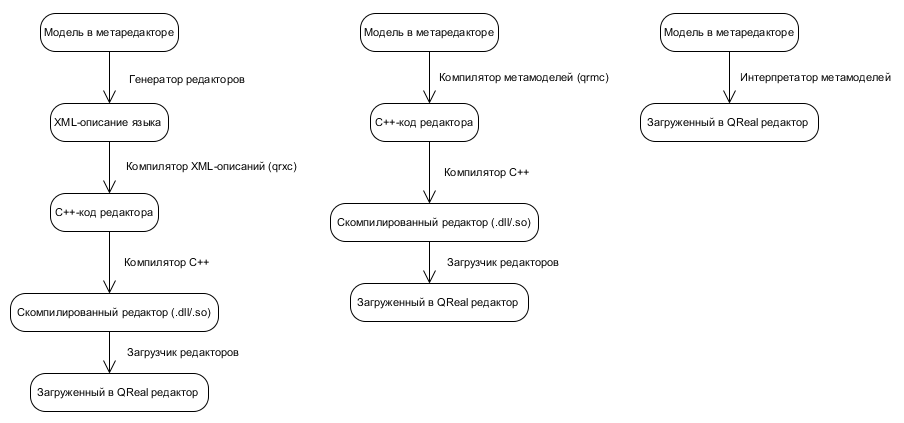
\includegraphics[width=0.7\textwidth]{editorGeneration.png}
    \caption{Способы генерации редактора}
    \label{editorGeneration}
  \end{center}
\end{figure}

Первый способ используется наиболее часто и предполагает использование промежуточного xml-формата представления метамодели. Пока метаредактора в QReal не существовало, все метамодели задавались вручную в xml-файлах, по которым затем порождался код на C++, компилировался, и подключался к основной части системы как динамически загружаемая библиотека. С появлением метаредактора в эту схему добавился генератор, порождающий по метамодели, хранящейся в репозитории, xml-файл с описанием метамодели. Второй способ был реализован позже и предполагает генерацию кода на C++ непосредственно по метамодели, без порождения промежуточного представления. Такой способ проще, но менее устойчив к изменениям в метаязыке --- если удалить какой-либо элемент метаязыка или даже какое-либо его свойство, старые метамодели, содержащие удалённый элемент, окажется невозможно загрузить и отредактировать. В xml-файлы в таких ситуациях изменения несложно внести вручную, редактировать вручную файлы с сохранёнными метамоделями гораздо сложнее. Поэтому второй способ не используется в процессе сборки QReal, а существует как альтернативный, до тех пор, пока не будет создано надёжного средства поддержки эволюции языков. На данный момент в процессе сборки QReal все плагины-редакторы (включая метаредактор) собираются из xml-файлов с метамоделями. Третий способ предполагает не генерацию по метамодели кода, реализующего редактор, а непосредственную интерпретацию метамодели в интерпретаторе, эмулирующем функциональность плагина-редактора. Такой способ технически наиболее удобен, поскольку для создания редактора не будет требоваться компилятор C++, и не требуется порождения никаких промежуточных представлений, однако же, интерпретируемый редактор работает медленнее сгенерированного. Интерпретатор может обладать рядом возможностей, недоступных сгенерированным редакторам, таким как модификация визуального языка "на лету", но на данный момент эти возможности в QReal не реализованы.

\subsection{Обсуждение}
Среду QReal:Robots вряд ли удалось бы разработать в столь короткие сроки вручную. Использование metaCASE-системы QReal позволило существенно упростить создание визуального языка и редактора диаграмм для него. Прототип языка был готов за несколько часов, так что уже после недели разработки первый функциональный прототип среды программирования, включающий в себя редактор диаграмм и интерпретатор, управляющий роботом по Bluetooth, был представлен специалистам по кибернетике. При создании языка наиболее затратным по времени оказался поиск подходящих иконок для блоков диаграммы. Создание метамодели языка с помощью метаредактора оказалось довольно быстрым, первая версия языка содержала порядка десятка блоков, находящихся друг с другом в несложных отношениях, и с тех пор язык лишь незначительно вырос, вся его метамодель в графическом виде помещается на один экран. Поскольку редактор диаграмм языка по метамодели генерируется автоматически, была возможность не только сэкономить время на разработке редактора, но и экспериментировать с языком, меняя блоки, их свойства и внешний вид. Кроме того, простота визуального представления синтаксиса языка дала возможность легко расширять и изменять его в дальнейшем, причём не только исходным авторам языка. Впоследствии разработка QReal:Robots была во многом передана студентам, которые без особых сложностей редактировали и расширяли язык по мере необходимости. Рассматривалась даже возможность позволить самим пользователям менять язык, например, дать возможность учителям информатики настраивать язык под конкретное занятие, но такая возможность до сих пор не была реализована в силу недоработанности средств метамоделирования в QReal.

Если синтаксис языка оказался хорошо формализуемым и процесс построения редактора языка по описанию синтаксиса удалось автоматизировать, то с семантикой ситуация оказалась хуже. Система QReal на момент разработки QReal:Robots не имела никаких средств описания семантики языка, так что вся инструментальная поддержка, включая интерпретатор диаграмм и генератор кода для заливки на робот, реализовывалась вручную, программированием на C++. Эта задача трудоёмка и сама по себе --- требовалось изучить систему прямых команд робота для управления им с компьютера, изучить API операционной системы робота для генерации кода для неё, наладить работу с Bluetooth, USB, кросскомпиляцию, прошивку робота, загрузку программы на робот и прочие проблемы, не автоматизируемые в принципе. Однако  некоторый код получился довольно шаблонным --- каждому блоку соответствовал некоторый класс на С++, реализовывавший его функциональность при интерпретации, и по крайней мере шаблоны для таких классов можно было бы генерировать автоматически по описанию языка. Интерпретатор в целом также мало связан конкретно с языком программирования роботов, так что, возможно, часть его можно было бы генерировать по описанию семантики языка, представленной в каком-то виде, а часть вынести в библиотеку и использовать в сгенерированном коде. Предполагается, что использование интерпретируемых языков программирования для описания части поведения интерпретатора позволило бы ускорить разработку, но эта идея ещё не была проверена.

Генератор кода представляется наиболее интересной целью для автоматизации, поскольку содержит много похожего от блока к блоку кода. Как и интерпретатор, генератор содержит неспецифичные для языка программирования роботов части, которые были бы применимы для всех визуальных языков с семантикой, похожей на семантику диаграмм активностей UML или блок-схем. Над автоматизацией создания генератора в QReal в данный момент ведётся работа, был создан язык описания правил генерации, берущий на себя многие типичные задачи, такие как обход графа модели и вывод текста. Тем не менее, такой язык не позволяет выполнять сложные алгоритмические действия, например, goto elimination или поиск переменных в математических выражениях для дальнейшей автоматической генерации блока объявления переменных.

Таким образом, результатом эксперимента по разработке системы визуального программирования с помощью metaCASE-системы стало то, что с помощью такого подхода можно создать систему, которая была бы не хуже разработанных вручную, и при этом время на разработку визуального редактора с помощью метамоделирования можно сократить в несколько десятков раз по сравнению с разработкой редактора вручную. Однако выигрыш при разработке и доведении до внедрения системы в целом оказался не таким значительным, как при разработке только редактора, потому как многие задачи принципиально неавтоматизируемы. В процессе эксперимента были выявлены типичные при разработке подобного рода систем задачи, которые можно в некоторой степени автоматизировать в metaCASE-системе, но их автоматизация требует дополнительных исследований. Большая часть таких задач требует изучения способов задания семантики визуальных языков. Однако даже сейчас DSM-подход показал себя полезным на практике, и представляется, что дальнейшие исследования в этом направлении смогут помочь эффективно создавать специализированные языки и среды программирования даже для гораздо более узких предметных областей и задач.

\section*{Заключение}
В результате применения описанного в статье подхода удалось разработать полноценную среду программирования роботов, которую оказалось возможным предложить школьникам и учителям в качестве замены используемых ныне в школах средств. QReal:Robots была представлена на "Открытых состязаниях Санкт-Петербурга по робототехнике" и на робототехническом фестивале "Робофест 2012" в Москве. В качестве доказательства применимости среды QReal:Robots к реальным задачам, решаемым школьниками, команда студентов приняла участие в соревнованиях в движении робота по линии с программой, реализованной целиком на QReal:Robots. Несмотря на то, что для студентов участие в соревнованиях стало практически первым опытом решения задач робототехники, им удалось показать довольно неплохие результаты, заняв места в середине таблицы, несмотря на то, что довольно многие участники использовали специально созданные для этой задачи роботы. QReal:Robots представлялся также в виде стендовых докладов, где вызвал большую заинтересованность у потенциальных пользователей. Было проведено анкетирование удобства пользовательского интерфейса, которое показало, что продукт достаточно хорош, чтобы вызывать у пользователей симпатию и желание им пользоваться.

Эксперимент показал применимость DSM-подхода для разработки средства визуального программирования, которое может распространяться как отчуждаемый продукт и рассчитано на аудиторию, не владеющую программированием. При этом использование средств автоматизации создания редакторов сэкономило много времени и усилий. Также в процессе эксперимента было выявлено несколько направлений, кажущихся перспективными для дальнейшей автоматизации.

\begin{thebibliography}{9001}

  \bibitem{shalitoEcl} \emph{Гуров В.С., Мазин М.А., Нарвский А.С., Шалыто А.А.} UML. SWITCH-техология. ECLIPSE. Информационно-управляющие системы. 2005. № 6. С. 12.

  \bibitem{qRealGithub} Домашняя страница проекта QReal на GitHub, URL: https://github.com/qreal/qreal 

  \bibitem{real1} \emph{Долгов П., Иванов А., Кознов Д., Лебедев А., Мурашева Т., Парфенов В., Терехов А.} Объектно-ориентированное расширение технологии RTST. // Записки семинара кафедры системного программирования ``CASE-средства RTST++’’. Вып. 1. CПб, Изд-во С.-Пб ун-та. 1998. С. 17--36.

  \bibitem{rtst1} \emph{Иванов А.Н., Кознов Д.В., Мурашова Т.С.} Поведенческая модель RTST. Записки семинара Кафедры системного программирования ``Case-средства RTST++’’. 1998. С. 37.

  \bibitem{msfDsm} \emph{Кознов Д.В.} Разработка и сопровождение DSM-решений на основе MSF. Системное программирование. Т. 3. № 1. 2008. С. 80--96.

  \bibitem{msfDsm2} \emph{Кознов Д.В., Ольхович Л.Б.} Визуальные языки проектов. Системное программирование. Т. 1. № 0. 2005. С. 148--167.

  \bibitem{videoDsl} \emph{Кознов Д.В., Перегудов А.Ф., Бугайченко Д.Ю., Чернятчик Р.И., Казакова А.С., Павлинов А.А.} Визуальная среда проектирования систем телевизионного вещания. Системное программирование. Т. 2. № 1. 2006. С. 142--168.

  \bibitem{student2} \emph{Комаров С.Н., Терехов А.Н., Граничина О.А.} Интегрированно-распределённая автоматизированная информационная система для крупного научно-образовательного учреждения. Вестник Санкт-Петербургского университета. Серия 10: Прикладная математика. Информатика. Процессы управления. 2008. № 1. С. 87--94. 

  \bibitem{dsmPlatforms} \emph{Павлинов А.А., Кознов Д.В., Перегудов А.Ф., Бугайченко Д.Ю., Казакова А.С., Чернятчик Р.И., Иванов А.Н.} О средствах разработки проблемно-ориентированных визуальных языков. Системное программирование. Т. 2. № 1. 2006. С. 116--141.

  \bibitem{sorKoz} \emph{Сорокин А.В., Кознов Д.В.} Обзор Eclipse Modeling Project. Системное программирование. 2010. Т. 5. № 1. С. 6--32. 

  \bibitem{qReal} \emph{Терехов А.Н., Брыксин Т.А., Литвинов Ю.В., Смирнов К.К., Никандров Г.А., Иванов В.Ю., Такун Е.И.} Архитектура среды визуального моделирования QReal. Системное программирование. Т. 4.  СПб.: Изд-во СПбГУ. 2000. С. 171--196

  \bibitem{rtst3} \emph{Терехов А.Н.} RTST --- технология программирования встроенных систем реального времени. Записки семинара Кафедры системного программирования "Case-средства RTST++". 1998. С. 3.

  \bibitem{student1} \emph{Терехов А.Н., Кияев В.И., Комаров С.Н.} Принципы информатизации системы управления в Санкт-Петербургском Государственном Университете. Вестник Санкт-Петербургского университета, Серия 8: Менеджмент. № 2. 2004. С. 151--200.

  \bibitem{filippov} \emph{Филиппов С.А.} Робототехника для детей и родителей, Наука, 2011. 264 С.

  \bibitem{shalito1} \emph{Шалыто А.А., Туккель Н.И.} Преобразование итеративных алгоритмов в автоматные. Программирование. 2002. № 5.

  \bibitem{shalito2} \emph{Шопырин Д.Г., Шалыто А.А.} Объектно-ориентированный подход к автоматному программированию. Информационно-управляющие системы. 2003. № 5. С. 29--39.

  \bibitem{rtst2} \emph{Парфенов В.В., Терехов А.Н.} RTST --- технология программирования встроенных систем реального времени. Системная информатика. 1997. С. 228.

  \bibitem{theBook} \emph{Kelly, S., Tolvanen, J.} Domain-Specific Modeling: Enabling Full Code Generation // Wiley-IEEE Computer Society Press. 2008. 448 p.

  \bibitem{kelly} \emph{Kelly, S., Tolvanen, J.-P.}, Visual domain-specific modeling: benefits and experiences of using metaCASE tools, in: Bezivin, J., Ernst, J. (Eds.), Proceedings of International workshop on Model Engineering, ECOOP 2000.

  \bibitem{kieburtz} \emph{Kieburtz, R., et al.} A software engineering experiment in software component generation, Proceedings of 18th International Conference on Software Engineering, Berlin, IEEE Computer Society Press, March, 1996.

  \bibitem{gmp} Graphical Modeling Project homepage, URL: http://www.eclipse.org/modeling/gmp/ 

  \bibitem{legoNxt} LEGO Mindstorms homepage, URL: http://mindstorms.lego.com/en-us/Default.aspx

  \bibitem{metaEditPlus} MetaEdit+ homepage, URL: http://www.metacase.com/ 

  \bibitem{mrds} Microsoft Robotics Developer Studio homepage, URL: http://www.microsoft.com/robotics/ 

  \bibitem{visio} Microsoft Visio homepage, URL: http://office.microsoft.com/ru-ru/visio/

  \bibitem{xmi} MOF/XMI specification, URL: http://www.omg.org/spec/XMI/2.4.1/ 

  \bibitem{nxtOsek} nxtOSEK homepage, URL: http://lejos-osek.sourceforge.net/ 

  \bibitem{robolabHome} Robolab home page, URL: http://www.ceeo.tufts.edu/robolabatceeo/ 

  \bibitem{robolab} \emph{Portsmore, Merredith} ROBOLAB: Intuitive Robotic Programming Software to Support Life Long Learning, APPLE Learning Technology Review, Spring/Summer 1999.

  \bibitem{weiss} \emph{Weiss, D., Lai, C. T. R.}, Software Product-line Engineering, Addison Wesley Longman, 1999.

  \bibitem{vsvmsdk} Visual Studio Visualization and Modeling SDK (was DSL SDK), URL: http://archive.msdn.microsoft.com/vsvmsdk 

  \bibitem{real2} \emph{Terekhov A.N., Romanovskii K.Yu., Koznov D.V., Dolgov P.S., Ivanov A.N.} RTST++: Methodology and CASE tool for the development of information systems and software for real-time systems. Programming and Computer Software. Vol. 25. № 5. 1999.С. 276--281.

\end{thebibliography}

\end{document}
